\section{Annisa Cahyani-1164066}
\subsection{Teori}
\begin{enumerate}
\item Mengapa File Teks Harus Dilakukan Tokenizer Besera Ilustrasi Gambar :
\begin{itemize}
\item Tokenizer :
\par Difungsikan untuk membuat vektor dari text. Lebih detailnya, tokenizer merupakan langkah pertama yang diperlukan dalam banyak tugas pemrosesan bahasa alami, seperti penghitungan kata.
\par
\par
\item Mengapa Text Harus Dilakukan Tokenizer ? :
\par Text harus dilakukan tokenizer agar dapat dirubah menjadi vektor dan dapat terbaca.
\par
\par
\item Ilustrasi Gambar : \ref{chapter-7-no-1-cahya}
\par
\begin{figure}[!hbtp]
\centering
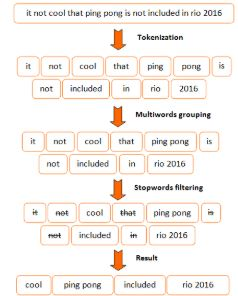
\includegraphics[scale=0.2]{figures/Chapter 7/1164066/Teori/chapter-7-no-1-cahya.jpg}
\caption{Tokenizer - cahya}
\label{chapter-7-no-1-cahya}
\end{figure}
\par
\end{itemize}
\par
\par
\par
\par
\item Konsep Dasar K Fold Cross Validation Pada Dataset Komentar Youtube Pada Kode Listing Beserta Dengan Ilustrasi Gambar :
\begin{itemize}
\item Code		:
\lstinputlisting[firstline=8, lastline=20, caption=K Fold Cross Validation,label={lst:7.0}]{src/1164066/chapter-7-2-cahya.py}
\item Penjelasan	: 
\par Untuk kejelasan dari StartifiedKFold yang dicontohkan ialah digunakan dan berisikan presentasi sampel untuk setiap kelas yang ada ( youtube).
\par
\end{itemize}
\par
\par
\par
\item Jelaskan Apa Maksud Kode Program For Train Dan Test In Splits Dilengkapi Dengan Ilustrasi Gambar :
\begin{itemize}
\item Penjelasan	:
\par Kode Program For Train dan Test In Splits sendiri digunakan ataupun difungsikan untuk pengujian. Pegujiannya yaitu menguji apakah setiap data pada dataset yang dieksekusi sudah di split.
\par 
\par
\end{itemize}
\par
\item Apa Maksud Kode Program\emph{train\_content = d['CONTENT'].iloc[train\_idx]} dan \emph{test\_content = d['CONTENT'].iloc[test\_idx]}. Dilengkapi Dengan Ilustrasi Gambar :
\begin{itemize}
\item Penjelasan	:
\par Maksud dari code program tersebut ialah difungsikan dalam pengambilan data pada kolom atau index CONTENT. index CONTENT tersebut merupakan bagian dari train\_idx dan test\_idx.
\par
\par
\end{itemize}
\par
\item Apa Maksud Dari Fungsi Tokenizer = Tokenizer(num words=2000) Dan Tokenizer.fit on texts(train content), Dilengkapi Dengan Ilustrasi Gambar :
\begin{itemize}
\item Penjelasan	:
\par  Fungsi dari Tokenizer diatas ialah untuk melakukan vektorisasi kata tentunya. Fungsi tokenizer ini mengeksekusi jumlah data yang akan diubah sebesar 2000 kata. Kemudian untuk  \emph{tokenizer.fit\_on\_texts(train\_content)} digunakan untuk melakukan fit tokenizer.
\par
\par
\end{itemize}
\par
\item Apa Maksud Dari Fungsi code berikut ( \emph{d\_train\_inputs = tokenizer.texts\_to\_matrix(train\_content, mode='tfidf')} dan \emph{d\_test\_inputs = tokenizer.texts\_to\_matrix(test\_content, mode='tfidf')} ), Dilengkapi Dengan Ilustrasi Kode Dan Atau Gambar :
\begin{itemize}
\item Penjelasan	:
\par Dapat dikatakan bahwa maksud dari codingan diatas ialah untuk variabel d\_train\_inputs dimana akan melakukan tokenizer dari bentuk teks ke / menjadi matrix dari data train\_content menggunakan mode matrik yaitu tfidf.
\par
\par
\end{itemize}
\par
\item Jelaskan Apa Maksud Dari Fungsi Berikut ( \emph{d\_train\_inputs = d\_train\_inputs/np.amax(np.absolute(d\_train\_inputs))} dan \emph{d\_test\_inputs = d\_test\_inputs/np.amax(np.absolute(d\_test\_inputs))} ) Kemudian Dilengkapi Dengan Ilustrasi Gambar :
\begin{itemize}
\item Penjelasan : 
\par Berdasarkan code diatas, menjelaskan bahwa fungsi tersebut akan membagi matrix tfidf yang sudah dieksekusi sebelumnya dengan amax. Amaxnya berfungsi dalam pengembalian maksimum array atau maksimum sepanjang sumbu.
\par
\par
\end{itemize}
\par
\par
\par
\item Jelaskan Apa Maksud Dari \emph{d\_train\_outputs = np.utils.to\_categorical(d['CLASS'].iloc[train]} Dan \emph{d\_test\_outputs = np\_utils.to\_categorical(d['CLASS'].iloc[test\_idx]} Dalam Kode Program Dilengkapi Dengan Ilustrasi Gambar :
\begin{itemize}
\item Penjelasan : 
\par Yang dimaksudkan dari kode program tersebut dapat dijelaskan bahwa fungsnya ditujukan untuk melakukan one-hot encoding.
\par One-hot encoding diambil dari 'CLASS'  dengan neuron bernilai satu nol(1,0) atau nol satu(0,1).
\par
\par
\par
\end{itemize}
\par
\par
\item Jelaskan Maksud Dari Fungsi Di Listing 7.2. Gambarkan Ilustrasi Neural Networknya Dari Model Kode Tersebut.
\begin{itemize}
\item Code :
\lstinputlisting[firstline=8, lastline=20]{src/1164066/chapter-7-9-cahya.py}
\item Penjelasan : 
\par Berdasarkan code tersebut, dimaksudkan atau ditujukan untuk melakukan pemodelan dengan sequential.Terdapat 512 neuron inputan dengan input shape 2000 vektor. Selanjutnya model dilakukan aktivasi dengan fungsi 'relu' untuk pemotongan bobot  sebesar 50 persen.Setelah itu muncullah outputan yang diaktivasi menggunakan fungsi softmax.
\par
\par
\end{itemize}
\par
\par
\par
\par
\item Jelaskan Maksud Dari Fungsi Di Listing 7.3. Dengan Parameter Berikut :
\begin{itemize}
\item Code :
\lstinputlisting[firstline=8, lastline=20]{src/1164066/chapter-7-10-cahya.py}
\item Penjelasan : 
\par Berdasarkan code tersebut , dimaksudkan bahwa model yang telah dibuat akan dicompile dengan menggunakan algoritma optimisasi, fungsi loss, dan fungsi metrik.
\par
\par
\end{itemize}
\par
\par
\par
\item Apa itu Deep Learning :
\begin{itemize}
\item Penjelasan :
\par Deep learning merupakan sub bidang pembelajaran mesin yang berkaitan dengan algoritma.
\par
\end{itemize}
\item Apa itu Deep Neural Network Dan Apa Bedanya Dengan Deep Learning :
\begin{itemize}
\item Penjelasan Deep Neural Network : 
\par Deep neural network adalah jaringan syaraf dengan tingkat kompleksitas tertentu, jaringan syaraf dengan lebih dari dua lapisan.
\par
\item Perbedaan Deep Neural Network Dan Deep Learning :
\par Perbedaan antara deep neural network dan deep learning terletak pada kedalaman model. deep learning adalah frasa yang digunakan untuk jaringan saraf yang kompleks. Kompleksitas ini disebabkan oleh pola yang rumit tentang bagaimana informasi dapat mengalir di seluruh model.
\par
\par
\end{itemize}
\par
\par
\item Bagaimana Perhitungan Algoritma Dengan Ukuran Stride (NPM mod3+1)x(NPM mod3+1) Yang Terdapat Pada Max Pooling :
\begin{itemize}
\item Penjelasan :
\par Konvolusi pada sebuah gambar dilakukan dalam pemrosesan image untuk menerapkan operator yang mempunyai nilai output dari piksel gambar yang berasal dari kombinasi linear.
\par
\item Langkah-langkah Algoritma Konvulasi Sesuai NPM : \ref{chapter-7-13-cahya}
\par
\par
\begin{figure}[!hbtp]
\centering
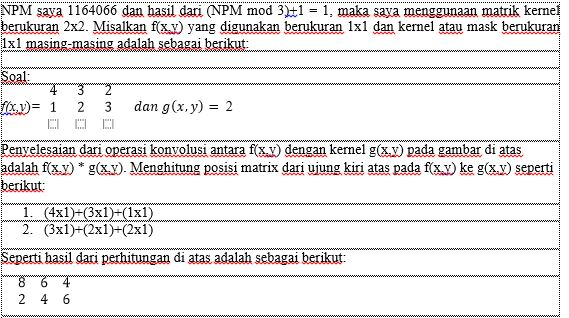
\includegraphics[scale=0.52]{figures/Chapter 7/1164066/Teori/chapter-7-13-cahya.jpg}
\caption{Langkah Algoritma Konvolusi- cahya}
\label{chapter-7-13-cahya}
\end{figure}
\par
\par
\end{itemize}
\end{enumerate}


\subsection{Praktek}
Penjelasan Tugas Harian 12 ( No 1-20 ).
\begin{enumerate}
\item Jelaskan Kode Program Pada Blok \# In[1]. Jelaskan Arti Dari Setiap Baris Kode Yang Dibuat Dan Hasil Keluarannya Dari Komputer Sendiri.
\begin{itemize}
\item Code Yang Digunakan : \ref{lst:praktek-chapter-7-1-cahya}.
\lstinputlisting[firstline=1, lastline=19,caption=File praktek-chapter-7-1-cahya.py.py, label={lst:praktek-chapter-7-1-cahya}]{src/1164066/praktek-chapter-7-1-cahya.py}
\par
\par
\item Penjelasan Code Perbaris	: 
\begin{enumerate}
\item Baris Code 1	: Memasukkan / Mengimport file csv
\item Baris Code 2	: Memasukkan module image sebagai pil\_image dari library PIL
\item Baris Code 3	: Memasukkan / mengimport fungsi keras.processing.image 
\end{enumerate}
\par
\item Hasil : \ref{chapter-7-in-1-cahya}
\par
\par
\begin{figure}[!hbtp]
\centering
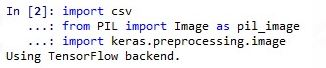
\includegraphics[scale=0.4]{figures/chapter-7-in-1-cahya.jpg}
\caption{Code Program Pada In [1] - cahya}
\label{chapter-7-in-1-cahya}
\end{figure}
\par
\par
\end{itemize}
\par
\par
\par
\item Jelaskan Kode Program Pada Blok \# In[2]. Jelaskan Arti Dari Setiap Baris Kode Yang Dibuat Dan Hasil Keluarannya Dari Komputer Sendiri.
\begin{itemize}
\item Code Yang Digunakan : \ref{lst:praktek-chapter-7-2-cahya}.
\lstinputlisting[firstline=1, lastline=19,caption=File praktek-chapter-7-2-cahya.py.py, label={lst:praktek-chapter-7-2-cahya}]{src/1164066/praktek-chapter-7-2-cahya.py}
\par
\par
\item Penjelasan Code Perbaris	: 
\begin{enumerate}
\item Baris Code 1	: Mendefinisikan variabel imgs tanpa parameter
\item Baris Code 2	: Mendefinisikan variabel classes tanpa parameter
\item Baris Code 3	: Membuka file HASYv2/hasy-data-labels.csv sebagai csvfile
\item Baris Code 4	: Mendefinisikan variabel csvreader yang memfungsikan pembacaan dari file csv
\item Baris Code 5	: Mendefinisikan variabel i dengan parameter 0
\item Baris Code 6	: Mengeksekusi baris dari pembacaan csv 
\item Baris Code 7	: Mengaplikasikan perintah "if" dengan ketentuan variabel i lebih besar dari angka 0
\item Baris Code 8	: Mendefinisikan variabel img yang mengubah image menjadi bentuk array (bilangan) dari file HASYv2
\item Baris Code 9	: Mendefinisikan variabel img tidak sama dengan nilai 255.0
\item Baris Code 10	: Mendefinisikan fungsi imgs.append dimana merupakan proses melampirkan atau menggabungkan data dengan file lain atau set data
\item Baris Code 11	: Mendefinisikan fungsi append kembali dari variabel classes dengan parameternya row[2].
\item Baris Code 12	: Mendefinisikan fungsi dimana i variabel i akan ditambah nilainya sehingga akan bernilai 1
\end{enumerate}
\par
\item Hasil : \ref{chapter-7-in-2-cahya}
\par
\par
\begin{figure}[!hbtp]
\centering
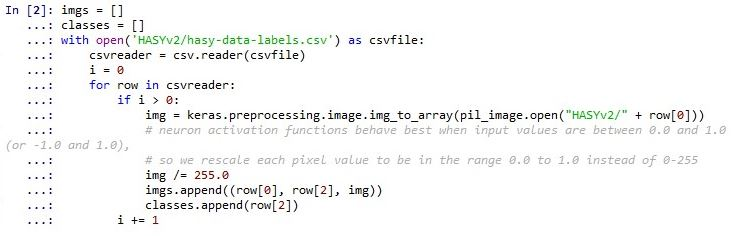
\includegraphics[scale=0.4]{figures/chapter-7-in-2-cahya.jpg}
\caption{Code Program Pada In [2] - cahya}
\label{chapter-7-in-2-cahya}
\end{figure}
\par
\par
\end{itemize}
\par
\par
\par
\item Jelaskan Kode Program Pada Blok \# In[3]. Jelaskan Arti Dari Setiap Baris Kode Yang Dibuat Dan Hasil Keluarannya Dari Komputer Sendiri.
\begin{itemize}
\item Code Yang Digunakan : \ref{lst:praktek-chapter-7-3-cahya}.
\lstinputlisting[firstline=1, lastline=19,caption=File praktek-chapter-7-3-cahya.py.py, label={lst:praktek-chapter-7-3-cahya}]{src/1164066/praktek-chapter-7-3-cahya.py}
\par
\par
\item Penjelasan Code Perbaris	: 
\begin{enumerate}
\item Baris Code 1	: Memasukkan  module random
\item Baris Code 2	: Melakukan pengocokan pada module random dengan parameter variabelnya imgs
\item Baris Code 3	: Memecah index dalam bentuk integer dengan mengkalikannilai 0,8 dan fungsi len yang akan mengembalikan jumlah item
\item Baris Code 4	: Mendefinisikan variabel train yang mengeksekusi imgs dengan pemecahan index awal pada data
\item Baris Code 5	: Mendefinisikan variabel test yang mengeksekusi imgs dengan pemecahan index akhir pada data
\end{enumerate}
\par
\item Hasil : \ref{chapter-7-in-3-cahya}
\par
\par
\begin{figure}[!hbtp]
\centering
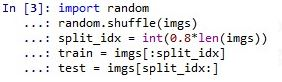
\includegraphics[scale=0.4]{figures/chapter-7-in-3-cahya.jpg}
\caption{Code Program Pada In [3] - cahya}
\label{chapter-7-in-3-cahya}
\end{figure}
\par
\par
\end{itemize}
\par
\par
\par
\item Jelaskan Kode Program Pada Blok \# In[4]. Jelaskan Arti Dari Setiap Baris Kode Yang Dibuat Dan Hasil Keluarannya Dari Komputer Sendiri.
\begin{itemize}
\item Code Yang Digunakan : \ref{lst:praktek-chapter-7-4-cahya}.
\lstinputlisting[firstline=1, lastline=19,caption=File praktek-chapter-7-4-cahya.py.py, label={lst:praktek-chapter-7-4-cahya}]{src/1164066/praktek-chapter-7-4-cahya.py}
\par
\par
\item Penjelasan Code Perbaris	: 
\begin{enumerate}
\item Baris Code 1	: Memasukkan / Mengimport library numpy sebagai np
\item Baris Code 2	: Mendefinisikan variabel train\_input dimana mengubah input menjadi sebuah array dari np dengan menggunakan fungsi list untuk mengkoleksikan data yang dipilih dan dapat diubah. 
\item Baris Code 3	: Mendefinisikan variabel test\_input dengan fungsi yang sama seperti train\_input yang membedakan hanya datanya / inputan yang diproses berasal dari variabel test
\item Baris Code 4	: Mendefinisikan variabel train\_output dimana mengubah keluaran menjadi sebuah array dari np dengan menggunakan fungsi list untuk mengkoleksikan data yang dipilih dan dapat diubah. 
\item Baris Code 5	: Mendefinisikan variabel test\_output dengan fungsi yang sama seperti train\_output yang membedakan hanya datanya / inputan yang diproses berasal dari variabel test
\end{enumerate}
\par
\item Hasil : \ref{chapter-7-in-4-cahya}
\par
\par
\begin{figure}[!hbtp]
\centering
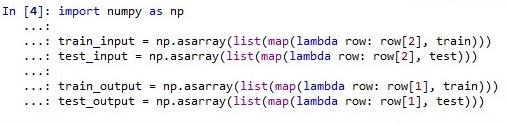
\includegraphics[scale=0.4]{figures/chapter-7-in-4-cahya.jpg}
\caption{Code Program Pada In [4] - cahya}
\label{chapter-7-in-4-cahya}
\end{figure}
\par
\par
\end{itemize}
\par
\par
\par
\item Jelaskan Kode Program Pada Blok \# In[5]. Jelaskan Arti Dari Setiap Baris Kode Yang Dibuat Dan Hasil Keluarannya Dari Komputer Sendiri.
\begin{itemize}
\item Code Yang Digunakan : \ref{lst:praktek-chapter-7-5-cahya}.
\lstinputlisting[firstline=1, lastline=19,caption=File praktek-chapter-7-5-cahya.py.py, label={lst:praktek-chapter-7-5-cahya}]{src/1164066/praktek-chapter-7-5-cahya.py}
\par
\par
\item Penjelasan Code Perbaris	: 
\begin{enumerate}
\item Baris Code 1	: Memasukkan modul / fungsi LabelEncoder dari sklearn.processing yang digunakan untuk menormalkan label dimana label encoder hanya didefinisikan dengan nilai antara 0 dan -1.
\item Baris Code 2	: Memasukkan modul / fungsi OneHotEncoder dari sklearn.processing yang digunakan untuk mendefinisikan fitur input dimana mengambil nilai dalam kisaran 0
\end{enumerate}
\par
\item Hasil : \ref{chapter-7-in-5-cahya}
\par
\par
\begin{figure}[!hbtp]
\centering
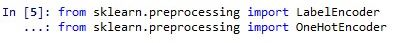
\includegraphics[scale=0.4]{figures/chapter-7-in-5-cahya.jpg}
\caption{Code Program Pada In [5] - cahya}
\label{chapter-7-in-5-cahya}
\end{figure}
\par
\par
\end{itemize}
\par
\par
\par
\item Jelaskan Kode Program Pada Blok \# In[6]. Jelaskan Arti Dari Setiap Baris Kode Yang Dibuat Dan Hasil Keluarannya Dari Komputer Sendiri.
\begin{itemize}
\item Code Yang Digunakan : \ref{lst:praktek-chapter-7-6-cahya}.
\lstinputlisting[firstline=1, lastline=19,caption=File praktek-chapter-7-6-cahya.py.py, label={lst:praktek-chapter-7-6-cahya}]{src/1164066/praktek-chapter-7-6-cahya.py}
\par
\par
\item Penjelasan Code Perbaris	: 
\begin{enumerate}
\item Baris Code 1	: Mendefinisikan variabel label\_encoder dengan penerapan modul / fungsi dari LabelEncoder
\item Baris Code 2	: Mendefinisikan variabel integer\_encoded dengan penerapan fungsi label\_encoder.fit\_transform (ekstrasi fitur object ) dari variabel classes dimana akan mengembalikan beberapa data yang diubah kembali
\end{enumerate}
\par
\item Hasil : \ref{chapter-7-in-6-cahya}
\par
\par
\begin{figure}[!hbtp]
\centering
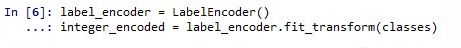
\includegraphics[scale=0.4]{figures/chapter-7-in-6-cahya.jpg}
\caption{Code Program Pada In [6] - cahya}
\label{chapter-7-in-6-cahya}
\end{figure}
\par
\par
\end{itemize}
\par
\par
\par
\par
\par
\par
\end{enumerate}


\subsection{Penanganan Error}
Penjelasan Tugas Harian 12 ( No 1-20 ).
\par
\par
